\documentclass[titlepage]{article}

\usepackage{graphicx}
\usepackage{hyperref}
\usepackage{indentfirst}
\usepackage{lipsum}
\usepackage{xcolor}

\begin{document}

	\thispagestyle{empty}
	\topskip0pt
	\vspace*{\fill}
		~\centerline{\textcolor{red}{\Huge{WORK IN PROGRESS}}}
		\newline\newline

		\begin{align*}
			\large{Known Issues}
			\begin{itemize}
				\item Adobe renders the 2.2 (The Parser) AST images oddly unless zoomed in
			\end{itemize}
		\end{align*}
	\vspace*{\fill}
	\newpage

	\title{Exploring Best Practices for the Creation of a Programming Language Ecosystem: A Case Study with ProtoSQL}
	\author{Brandon Browning}
	\maketitle

	\begin{abstract}

		Developing a programming language is a process full of managing many different forms of complexity.  This project is an experiment in managing the problems that may arise in the development of an ecosystem for a new programming language; it is meant to explore and evaluate the best practices through the creation of a full language.  This will result in an industrial-strength and full-featured tool chain, including a parser, optimizer, and compiler.  The parser will adhere to the language grammar, generate descriptive error messages, and supply an Abstract Syntax Tree (AST) to the optimizer.  The optimizer will then go through the tree and rewrite pieces as it sees fit, generally to improve performance.  Then the compiler, here a cross-compiler, will take the AST and output corresponding SQL code.

	\end{abstract}

	\section{Insight}

		This project started out with a deep curiosity into how languages are defined, and how people manage the tooling around them.  To somebody who is unfamiliar with workings of parsers and compilers, it seems like such an immense and magical process to have code that turns code into code.  It's always a bit magical, but I hope through this paper to show how the field of Computer Science has dealt with this problem, and why it's not as painful as one would think.

		First I'll go over some of the ideas behind programming languages; such as why new ones should be created, the ecosystem surrounding them, and how different ways they're implemented.  Then I'll describe the process behind the creation of ProtoSQL; including the difficulties faced, the benefits of some of the practices employed, and the overall experience and outcome of working on a new programming language.

	\section{Overview of Creating a New Language}

		Languages are usually created because there's some kind of problem one would like to solve; such as wanting to work at an abstraction level between two other languages, or a completely different way of thinking to some established standard.  Over time, the strengths and weaknesses of a language begin to show.  The weaknesses are not necessarily oversights by the original designer, but more intricacies that are brought out over time by heavy usage of the language.  Due to this phenomenon, the development of new languages serves an important role in the evolution of software.

		\subsection{First Steps}

			The first part of the process towards the foundation of a new programming language, almost out of necessity, is to develop the syntax and semantics of how the language will function.  There's an already existing domain of problem that the creator wants to solve, so they must think on the constructs used to solve that problem, and how they will fit together.  For example, if somebody wanted to create a language for a hand-held algebra system, they'd have to consider brevity and ease of entry as design goals.  They may opt to limit the feature set and complexity of the language as it's probably aimed at beginners, and the limited input versus a desktop-based system would be a significant factor.  At this point, many of the details aren't known, but the high-level design starts coming in to play which heavily dictates the initial direction of the language.

		\subsection{The Parser}

			Usually the first part of a new programming language ecosystem to be implemented is the parser.  The construction of a parser helps solidify the correctness of the grammar, lets you start working on and provides a basis for the compiler, and helps iron out and explore the grammar.  If the language hasn't been carefully scoured over before work on the parser begins, then problems in the grammar naturally surface during work on the parser.

			Now what exactly does the parser do?  The parser is the engine that turns the source text, or the source material for the entire process, into a structure fed through the rest of the system until completion; this structure is known as an Abstract Syntax Tree (AST).  The AST is a representation of the grammar in the form of a manipulatable data structure.  The primary purpose of the parser is then to turn the source text into its corresponding AST.

			The AST could be visualized as a tree or graph data structure which is common in Computer Science, and where the name comes from; however, this is beyond the scope of the paper.  Essentially, It is a hierarchal structure of the pieces of the language that the source text demonstrates.  For example, here's a simple arithmetic expression:
			\newline

			~\centerline{\Large{$x + 5$}}
			\newline

			This could be represented graphically, slightly simplified, as the following..
			\footnote{AST Graphics generated from \href{http://www.gliffy.com}{gliffy.com} and manipulated with \href{http://www.getpaint.net/}{Paint.NET}}
			\newline

			~\centerline{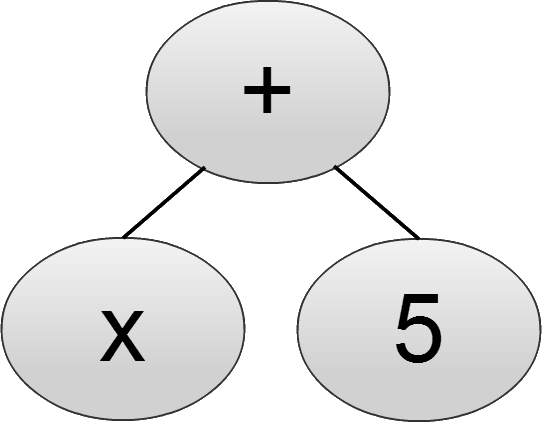
\includegraphics[scale=.3]{SimpleAST.png}}
			\newline

			An more complex example, as code instead of mathematics:
			\newline

			~\centerline{\Large{$f(g(x)) + \frac{1}{2}$}}
			\newline

			The AST representation would resemble the following..
			\footnotemark[\value{footnote}]
			\newline

			~\centerline{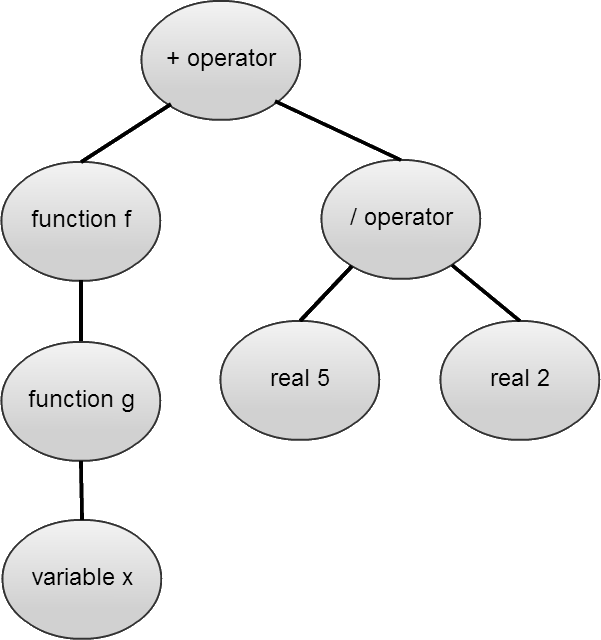
\includegraphics[scale=.5]{PseudocodeAST.png}}
			\newline

			To be continued..

\end{document}